\subsection{Data}

Following in the footsteps of much previous work in this area \cite{lappas2009finding, kargar2011discovering, bhowmik2014submodularity}, we run our experiments on the DBLP dataset.
DBLP consists of a long list of academic publications in computer science.
We take each author to represent a node; authors that appear as coauthors are considered to have lower communication cost.
Specifically, the communication cost between authors $ A $ and $ B $ is given as,
\begin{equation}\label{eqn:ccost}
1 - \frac{| \left\{ p \in P, author(A, p) \land author(B, p) \right\} |}{| \left\{ p \in P, author(A, p) \lor author(B, p) \right\} |}
\end{equation}
In equation \ref{eqn:ccost} $ P $ denotes the set of all papers in the database, and the predicate $ author(X, p) $ is true precisely when author $ X $ appears as an author on paper $ p $.

The skills of an author correspond to the ``key words'' of the titles of the papers on which they are authors; while we were unable to find a precise definition of ``key word'' in any previous work, we opted to exclude ``connecting'' words like ``and'', ``the'', ``of'', etc. from the space of possible skills.
To determine the skill distribution, we assumed independence between skills, such that the probability of a particular skill $ s $ appearing in a task is $ \frac{count(s)}{\sum_{s' \in \mathcal{S}} count(s')} $, where $count(s)$ denotes the number of authors in the dataset that have the skill $s$.
At runtime, to achieve tractability of the inference, the calculation of expectation over tasks was simplified by applying a threshold of $0.005$. Skills that have probabilities below the threshold are deemed noisy and their probabilities were set to $0.0$.

In similar fashion to the previous studies on the Team Formation problem, we filter papers to those published in the following venues: "journal/sigmod", "conf/vldb", "conf/icde", "conf/icdt", "conf/edbt", "conf/pods", "conf/kdd", "conf/www", "conf/sdm", "conf/pkdd", "conf/icdm", "conf/icml", "conf/ecml", "conf/colt", "conf/uai", "conf/soda", "conf/focs", "conf/stoc", "conf/stacs".
Then, also in keeping with previous work, we filtered authors to those who had 3 or more publications.
In an additional step, in distinction to previous work, we limit authors to a maximum of 10 skills.
The space of all possible skills, $ \mathcal{S} $, is limited only to those skills that are possessed by at least one author in the remaining set.

\subsection{Configuration}

Recall that in our objectives we have two layers of optimization. In section \ref{sec:algos} we stated that four possible candidate algorithms to optimize over the objectives. The inner optimization can be performed using the greedy choice of ratio of submodular function (RS), as proposed by the authors of \cite{bai2016algorithms}. Alernatively one can simply use Monte Carlo (MC) search for that. For the outer optimization we can again use MC or perform a greedy selection. In the following table, the number of samples used for the Monte Carlo search for the inner and outter optimization subroutines are listed for all four possible choices. The first option denotes the option chosen for the outer optimization, the second corresponds to the inner one.

\begin{center}
	\begin{tabular}{ c|c|c } 
		 & outter & inner \\
		\hline
		\texttt{greedy\_rs} &  &  \\
		\texttt{mc\_rs} & 20 &  \\
 		\texttt{greedy\_mc} &  & 200 \\
 		\texttt{mc\_mc} & 50 & 100 \\
	\end{tabular}
\end{center}

In the following experiments, we keep constant the size of the initial organization to 10 individuals. 
We also considered setting the starting number of individuals in the organization to 100, but found that the overall trends were the same, only with a greater separation between the best- and worst-performing algorithms, and at substantial runtime cost for the less efficient algorithms.

\subsection{Effect of hiring pool size on solution quality}
\label{section:num-candidates}

\begin{figure}[h!]
	\centering
	(a) 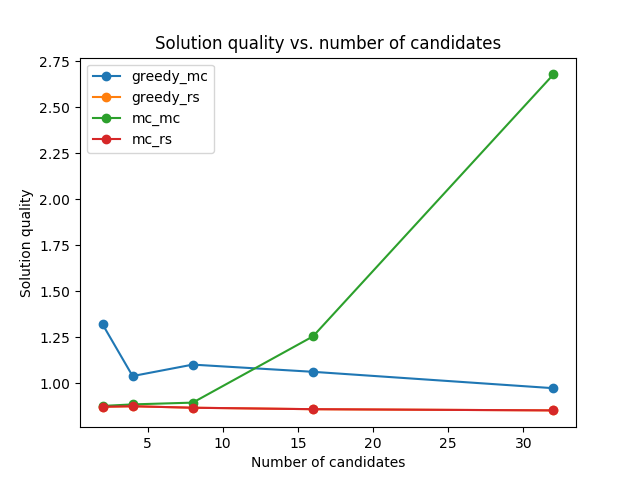
\includegraphics[width=0.6\textwidth]{figs/num_candidates_multi_ground_set_plot.png}
	
	(b) 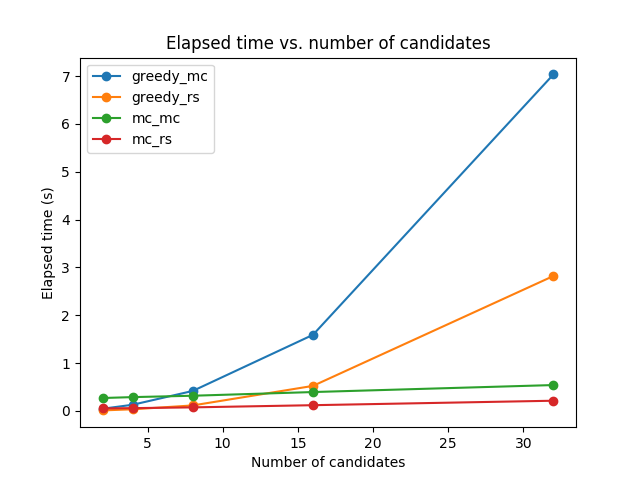
\includegraphics[width=0.6\textwidth]{figs/num_candidates_multi_ground_set_times_plot.png}
	\caption{(a) Note that as HireMax is implemented as a minimization problem, a lower solution quality is better. (b) Elapsed time is wall clock time measured in seconds.}
	\label{fig:num-candidates}
\end{figure} 

The first variable under which we wish to measure the performance of our heuristics is under varying recruiting pool sizes.
We consider hiring pools of sizes 2, 4, 8, 16, and 32 persons.
For each size of hiring pool, we arbitrarily set the hiring budget to be half the number of potential hires.

For each hiring pool size, we consider 5 different randomly-drawn ground sets of individuals to constitute the initial organization, and for each of these, we randomly sample 5 different sets of candidates of the appropriate size.
This gives a total of 25 random trials for each hiring pool size.

Results for this experiment are shown in Figure \ref{fig:num-candidates}.
The first thing to notice is that aside from \texttt{mc\_mc}, all algorithms tested are fairly robust to orders-of-magnitude increases in the number of candidates.
The degradation in the performance of \texttt{mc\_mc} may be explained by the fact that it acts in a sort of ``scattershot'' fashion, randomly picking points from space to evaluate.
Clearly, the bigger this space, the worse this will perform.

Next, we notice that \texttt{mc\_rs} and \texttt{greedy\_rs} have practically identical performance.
This may be explained by the fact that they both make repeated calls to the same inner optimization subroutine, i.e. the \textsc{GreedRatio} function for RS minimization (Algorithm \ref{alg:greed-ratio}).
Although the outter procedures in charge of selecting subsets of candidates to evaluate are different (one is a simple greedy search, the other uses a na\"ive Monte Carlo simulation), it seems that there is not much variation between the values of different possible subsets.
This makes sense when one considers that the distribution of skills across authors in this dataset is fairly sparse (average task frequency of $ 3.7567 \times 10^{-4} $), so it is often not worth the cost of hiring additional authors beyond the first one, who provides the bulk of the contribution to the utility.
By definition, the simple greedy search will start by considering the value of hiring the single candidate who provides the greatest marginal gain to the company.
Therefore, so long as the Monte Carlo simulation draws at least one sample containing that individual, the inner \textsc{GreedRatio} subroutine will find the value of the team consisting of only that individual, regardless of the other candidates being considered at the same time.

Another striking observation to be made from Figure \ref{fig:num-candidates}(a) is that the curves for \texttt{mc\_rs} and \texttt{greedy\_rs} are virtually flat.
This is consistent with our hypothesis above, that the first greedily-chosen candidate makes the biggest impact upon the organization, and this is precisely the candidate first selected by the \textsc{GreedRatio} subroutine.

Figure \ref{fig:num-candidates}(b) reveals that these greedy algorithms come with a tradeoff in scalability.
In this plot, the outter subroutine is the one that determines performance: both the algorithms that use Monte Carlo search to select candidate subsets to evaluate, have a very shallow slope.
This makes sense, since they were parameterized to always perform the same number of samples, regardless of the number of candidates.
On the other hand, the scalability of the outter greedy subroutine is called into question by the accelerating slopes of the algorithms using it.

Taking into consideration both Figure \ref{fig:num-candidates}(a) and \ref{fig:num-candidates}(b), it seems that the \texttt{mc\_rs} algorithm offers the best tradeoff between performance and scalability.

\subsection{Effect of budget tightness on solution quality}

\begin{figure}[h!]
	\centering
	(a) 	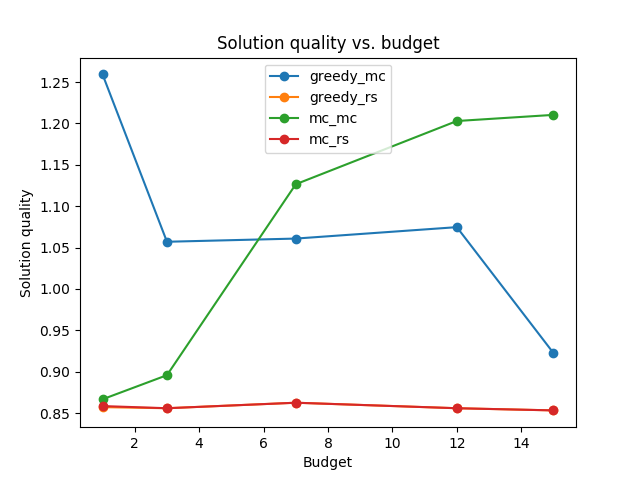
\includegraphics[width=0.6\textwidth]{figs/budget_results_multi_ground_set_plot.png}
	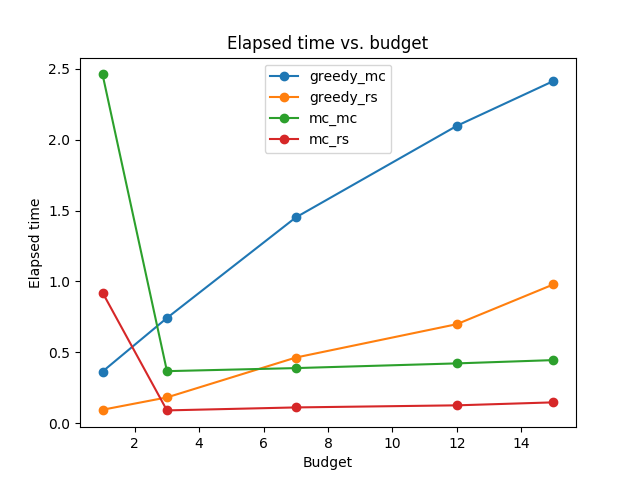
\includegraphics[width=0.6\textwidth]{figs/budget_results_multi_ground_set_time_plot.png}
	\caption{(a) Note that as HireMax is implemented as a minimization problem, a lower solution quality is better. (b) Elapsed time is wall clock time measured in seconds.}
	\label{fig:budget}
\end{figure}

Next, we consider the tightness of the constraint placed by the hiring budget.
The intuition here is that on the one hand, few subsets of potential hires will satisfy very strict constraints, and so few evaluations of the objective function will need to be made; hence, one might expect the optimization problem to be easier here.
On the other hand, very loose constraints make it easier to hire more people, making it less likely that we'll erroneously neglect to hire one of the more valuable candidates.
In between these two extremes, one would expect that there lies some sort of phase transition, within which region constrained optimization problems are particularly difficult to solve.

Hence, we investigate the effect of varying budget size on solution quality.
We keep the size of the candidate pool consistent at 16 candidates, and select from a hiring budget of 1, 3, 7, 12, or 15 candidates.
All other parameters are the same as those in Section \ref{section:num-candidates}.
Results are presented in Figure \ref{fig:budget}.

The trends in Figure \ref{fig:budget}(a) are similar to those seen in Figure \ref{fig:num-candidates}(a) (analyzed above), with the biggest apparent difference being in the scaling of the y-axis.
This is simply a result of not considering the larger team size of 32, which was responsible for the sharp jump in solution badness for \texttt{mc\_mc} in Figure \ref{fig:num-candidates}(a).

Slightly more interesting is the left side of Figure \ref{fig:budget}(b), where the two algorithms employing Monte Carlo search for candidate subset selection experience a sharp spike.
This is explainable by the na\"iveness of the sampling algorithm they employ---if a sample is drawn that violates the budget constraint (i.e. too many candidates are included in it), then that sample is thrown out and a new one is generated, etc.
Samples that are rejected in this way are not counted towards the total number of samples required for that algorithm.
For tight constraints, such as hiring only a single candidate out of 16, this means that most samples will be thrown out, and hence the algorithm will spend a long time searching for samples that satisfy the budget constraint.

Once again, \texttt{mc\_rs} emerges as the victor in terms of both optimality and efficiency.
